\chapter{Διπλά συστήματα \& Μεταβλητοί αστέρες}
\label{ch:Chapter7}

\section{Διπλά συστήματα αστέρων}


\underline{Διπλό σύστημα αστέρων}: {\color{blue}δύο αστέρες που αλληλεπιδρούν βαρυτικά και το σύστημα είναι δέσμιο.} Αν ένας αστέρας έχει μεγάλη ταχύτητα και περάσει από την γειτονιά ενός άλλου αστέρα, τότε τα 2 αστέρια θα αλληλεπιδράσουν βαρυτικά μεν, αλλά το σύστημα δεν θα είναι δέσμιο.

Το ότι το σύστημα είναι δέσμιο σημαίνει ότι η ενέργεια του συστήματος είναι αρνητική (θετική κινητική ενέργεια προφανώς, αλλά αρνητική δυναμική). Επίσης ισχύουν τα εξής:

\begin{itemize}
    \item Οι αστέρες εκτελούν ελλειπτικές τροχιές γύρων από το κέντρο μάζας (ΚΜ) του συστήματος.
    \item Το επίπεδο και η περίοδος της τροχιάς είναι κοινά και για τα δύο αστέρια.
    \item το ΚΜ βρίσκεται στην ευθεία που ενώνει τα δύο αστέρια, και η θέση του σ' αυτή καθορίζεται από την σχέση:
        \begin{equation}
            \label{eq:center_mass}
            \frac{a_B}{a_A} = \frac{M_A}{M_B}
        \end{equation}
        όπου $a_A, a_B$ είναι οι αποστάσεις των αστέρων από το ΚΜ.
    \item Για την περίοδο των τροχιών των αστέρων, P, ισχύει ο 3ος νόμος του Kepler
        \begin{equation}
            \label{eq:Kepler_third_law}
            P^2 = \frac{4\pi^2}{G}a^3 \frac{1}{(M_A + M_B)}
        \end{equation}
        όπου $a$ είναι ο μεγάλος ημιάξονας της τροχιάς της \textit{σχετικής} θέσης των δύο αστέρων.
\end{itemize}

Αν γνωρίζουμε λοιπόν τα χαρακτηριστικά του συστήματος (γωνία κλίσης επιπέδου τροχιάς, $P, a_B, a_A, a$) τότε έχουμε ένα σύστημα 2 εξισώσεων (τις σχέσεις \eqref{eq:center_mass} και \eqref{eq:Kepler_third_law}) για 2 αγνώστους ($M_A$, $M_B$).  Έτσι, μπορούμε να υπολογίσουμε τις μάζες των δύο αστέρων.






\subsection{Κατηγορίες διπλών συστημάτων}
Τα διπλά συστήματα αστέρων κατηγοριοποιούνται ανάλογα με την φαινόμενη απόσταση των δύο αστέρων και τη δυνατότητα διαχωρισμού τους από τα γήινα τηλεσκόπια. Έτσι προκύπτουν οι κάτωθι κατηγορίες.

\subsubsection{Οπτικά διπλοί αστέρες}
Τα συστήματα αυτά αποτελούνται από διπλούς αστέρες τα μέλη των οποίων είναι ορατά με γυμνό μάτι ή τηλεσκόπιο ως διακριτοί αστέρες. Είναι συνήθως κοντινά συστήματα με μεγάλες περιόδους περιστροφής και μεγάλες αποστάσεις μεταξύ των μελών του συστήματος.
Ένα τέτοιο σύστημα μπορεί να αποτελεί \textit{πραγματικά} διπλό σύστημα αστέρων όπως το έχουμε ορίσει, αλλά επίσης μπορεί δύο αστέρες να βρίσκονται σε τελείως διαφορετικές αποστάσεις από τη Γη και να φαίνεται σαν ένα διπλό σύστημα επειδή προβάλλεται πάνω στο επίπεδο της ουράνιας σφαίρας. Αυτοί ονομάζονται \textit{φαινομενικά} διπλοί αστέρες.

Η θεωρητική διακριτική ικανότητα, $\omega_{\text{min}}$, ενός οπτικού οργάνου εξαρτάται από το μήκος κύματος της παρατήρησης και τη διάμετρο, $D$, του αντικειμενικού φακού (ή κατόπτρου) σύμφωνα με τη σχέση:
\begin{equation}
    \omega_{\text{min}} = 1.22 \frac{\lambda}{D}
\end{equation}

\subsubsection{Μη-οπτικά διπλοί αστέρες}
Η κατηγορία αυτή διπλών αστέρων είναι αυτή των οποίων το ένα μέλος δεν διακρίνεται επειδή είναι εξαιρετικά αμυδρό. Η κατηγορία αυτή χωρίζεται σε 4 υποκατηγορίες ανάλογα με τη μέθοδο που χρησιμοποιούμε για να αντλήσουμε πληροφορίες από ένα τέτοιο σύστημα.

\begin{enumerate}[label=(\Roman*)]
    \item \textbf{Φασματοσκοπικά διπλοί αστέρες (spectroscopic binaries)} \\
    Από τον 3ο νόμο του Kepler (σχέση \eqref{eq:Kepler_third_law}) προκύπτει ότι όταν ο μεγάλος ημιάξονας της τροχιάς των μελών του συστήματος είναι μικρός, οι ταχύτητες περιφοράς των αστεριών γύρω από το κοινό ΚΜ είναι μεγάλες, με άμεσο αποτέλεσμα να μετατοπίζονται οι φασματικές γραμμές του συστήματος λόγω του φαινομένου Doppler.
        \begin{figure}
            \centering
            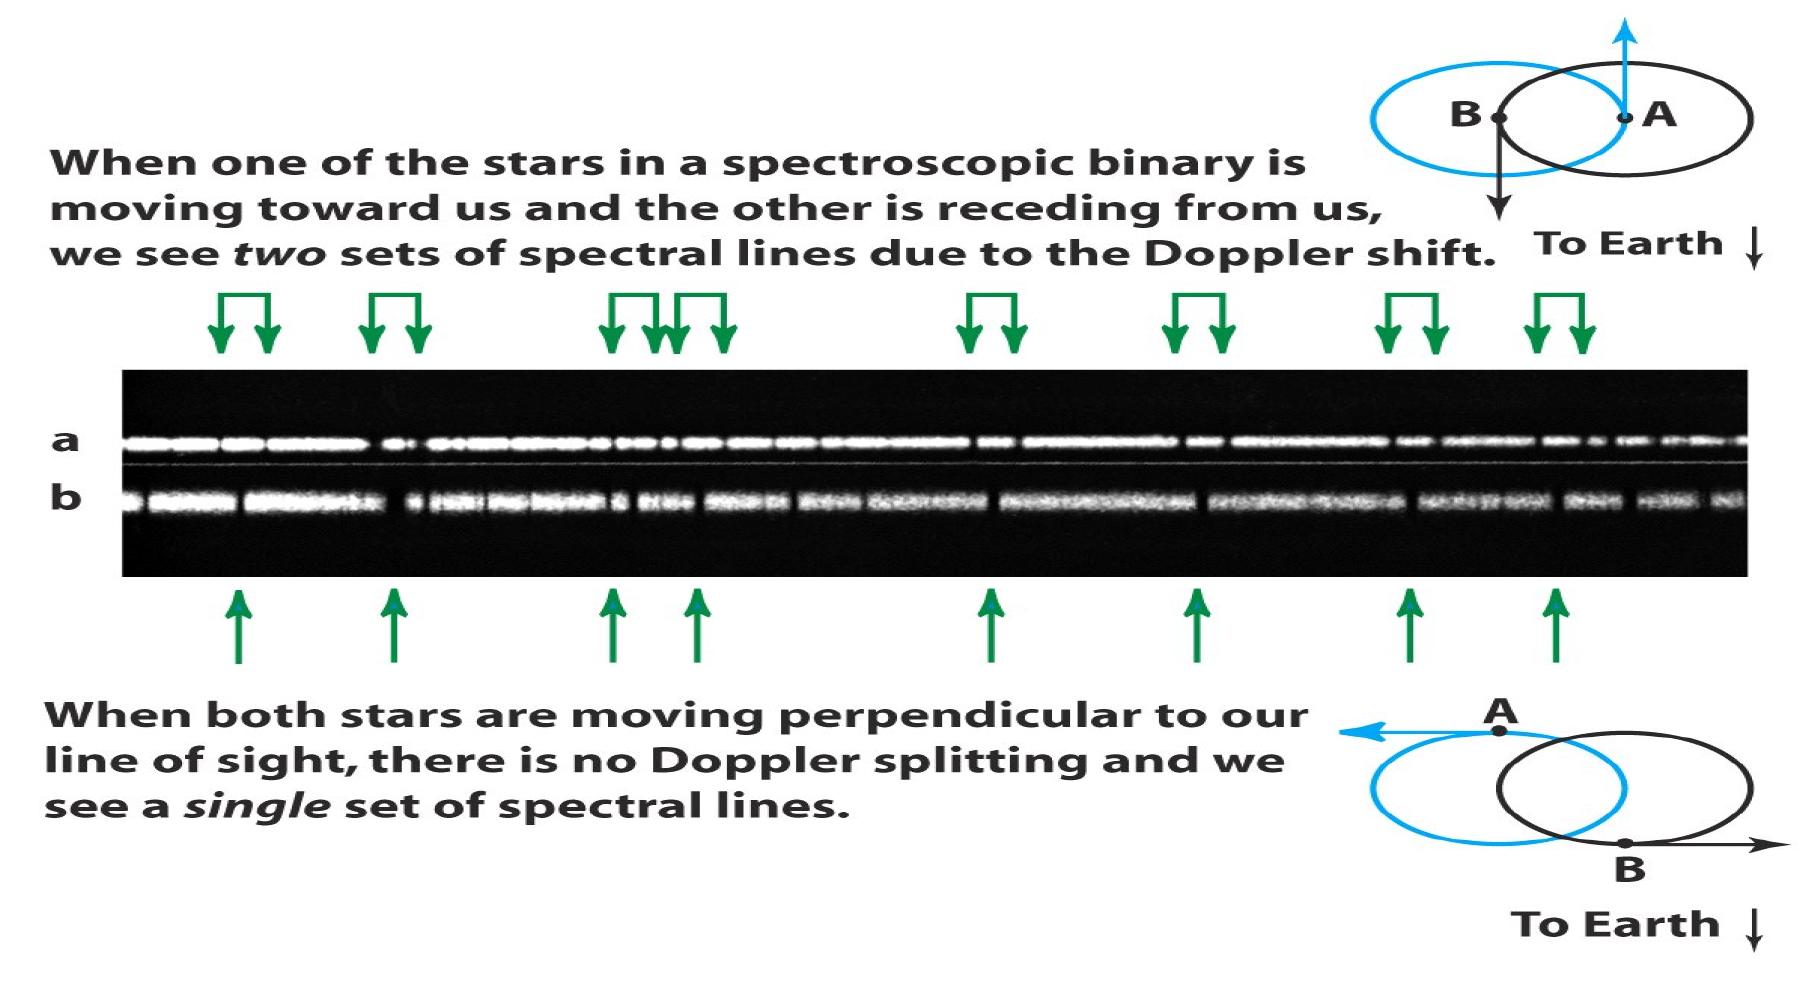
\includegraphics[width=\linewidth]{Figures/spectroscopic_binary.png}
            \caption{Φασματοσκοπικά διπλό σύστημα αστέρων.}
            \label{fig:spectroscopic_binary}
        \end{figure}
    Από το φάσμα που παίρνουμε, βλέπουμε ότι περιέχει γραμμές που ανήκουν σε δύο αστέρες (αν οι λαμπρότητες των μελών είναι συγκρίσιμες) ή μόνο σε έναν αστέρα (αν η λαμπρότητα του ενός είναι πολύ μεγαλύτερη από του άλλου). Κάθε φασματική γραμμή ``ταλαντώνεται'' περιοδικά γύρω από ένα μέσο μήκος κύματος. Προφανώς οι φασματικές γραμμές μετατοπίζονται προς το ερυθρό όταν ο αντίστοιχος αστέρας βρίσκεται στο τμήμα της τροχιάς που απομακρύνεται από τη Γη, και προς το κυανό όταν βρίσκεται στο τμήμα της τροχιάς που προσεγγίζει τη Γη (σχήμα \ref{fig:spectroscopic_binary}). Επειδή οι 2 αστέρες βρίσκονται πάντα σε αντιδιαμετρική θέση ως προς το ΚΜ, όταν οι φασματικές γραμμές του ενός αστέρα είναι μετατοπισμένες προς το ερυθρό, οι φασματικές γραμμές του άλλου είναι μετατοπισμένες προς το κυανό και αντίστροφρα. Οι περισσότεροι γνωστοί διπλοί αστέρες είναι φασματοσκοπικά διπλοί χωρίς αυτό να σημαίνει ότι δεν μπορούν να ανήκουν ταυτόχρονα και σε κάποια άλλη κατηγορία.
        
    Από τον χρόνο που χρειάζεται για να έχουμε δύο διαδοχικές ταυτήσεις των φασματικών γραμμών, μπορούμε να βρούμε την \textit{περίοδο} του συστήματος. Επίσης, ξέρουμε ότι η μετατόπιση από τη θέση ισορροπίας (της φασματικής γραμμής) εξαρτάται από τη συνιστώσα της \textit{ταχύτητας κατά μήκος της γραμμής παρατήρησης} (line of sight). Δεν έχουμε και τις 3 συνιστώσες για το διάνυσμα της ταχύτητας. Μέσω αυτής της συνιστώσας της ταχύτητας μπορούμε να βρούμε και την απόσταση των δύο σωμάτων μεταξύ τους (ανάλογα με το πως αλλάζει το πλάτος της ταχύτητας).
        
    \underline{Σημείωση}: Τα μήκη κύματος στα οποία εμφανίζονται οι μετατοπισμένες γραμμές απορρόφησης δεν αντιστοιχούν σε κανένα χημικό στοιχείο που μπορεί να δώσει μετάπτωση από μία ενεργειακή στιβάδα σε κάποια άλλη και να παράξει αυτά τα μήκη κύματος.
        
    Μέσω της μελέτης των φασματοσκοπικά διπλών αστέρων \textit{δεν} είναι δυνατόν να υπολογισθεί η μάζα των αστέρων του συστήματος, παρά μόνο ο λόγος των μαζών τους και το γινόμενο της κάθε μάζας επί την άγνωστη ποσότητα $\sin^3 i$, όπου $i$ είναι η γωνία κλίσης του επιπέδου της τροχιάς του διπλού συστήματος (σχήμα \ref{fig:inclination_angle}).
        \begin{figure}
            \centering
            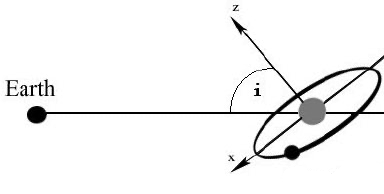
\includegraphics[scale=0.8]{Figures/inclination.jpg}
            \caption{Η γωνία κλίσης $i$, του επιπέδου της τροχιάς ενός διπλού συστήματος αστέρων.}
            \label{fig:inclination_angle}
        \end{figure}
        
    \item \textbf{Εκλειπτικά διπλοί αστέρες (ecliptic binaries)}\\
    Όταν το επίπεδο της τροχιάς των δύο αστέρων είναι σχεδόν παράλληλο με τη διεύθυνση παρατήρησης, δηλαδή η γωνία κλίσης $i \simeq 90^{\circ}$, και η απόσταση μεταξύ των μελών του συστήματος είναι πολύ μικρή, τότε κατά την περιφορά τους γύρω από το ΚΜ, τα 2 μέλη διέρχονται διαδοχικά το ένα μπροστά από το άλλο έτσι ώστε το ένα να καλύπτει τμήμα (ή και το σύνολο) του φαινόμενου δίσκου του άλλου, προκαλώντας μερικές ή όλικές εκλείψεις.
    Η ύπαρξη του ζεύγους συνεπάγεται από τις περιοδικές μεταβολές (αυξομειώσεις) της φαινόμενης λαμπρότητας του --φαινομενικά απλού-- αστέρα, η οποία μειώνεται κατά τη διάρκεια της έκλειψης.
    
    Κατά τη διάρκεια μίας περιφοράς συμβαίνουν δύο εκλείψεις, ανάλογα με το ποιό αστέρι βρίσκεται μπροστά από το άλλο και ως εκ τούτου παρουσιάζονται δύο ελάχιστα λαμπρότητας (σχήμα \ref{fig:eclipsing_binary}). Τα δύο αυτά ελάχιστα διαφέρουν γενικά ως προς το πλάτος και το βάθος, ανάλογα με τη λαμπρότητα των μελών του συστήματος.
        \begin{figure}[h]
            \centering
            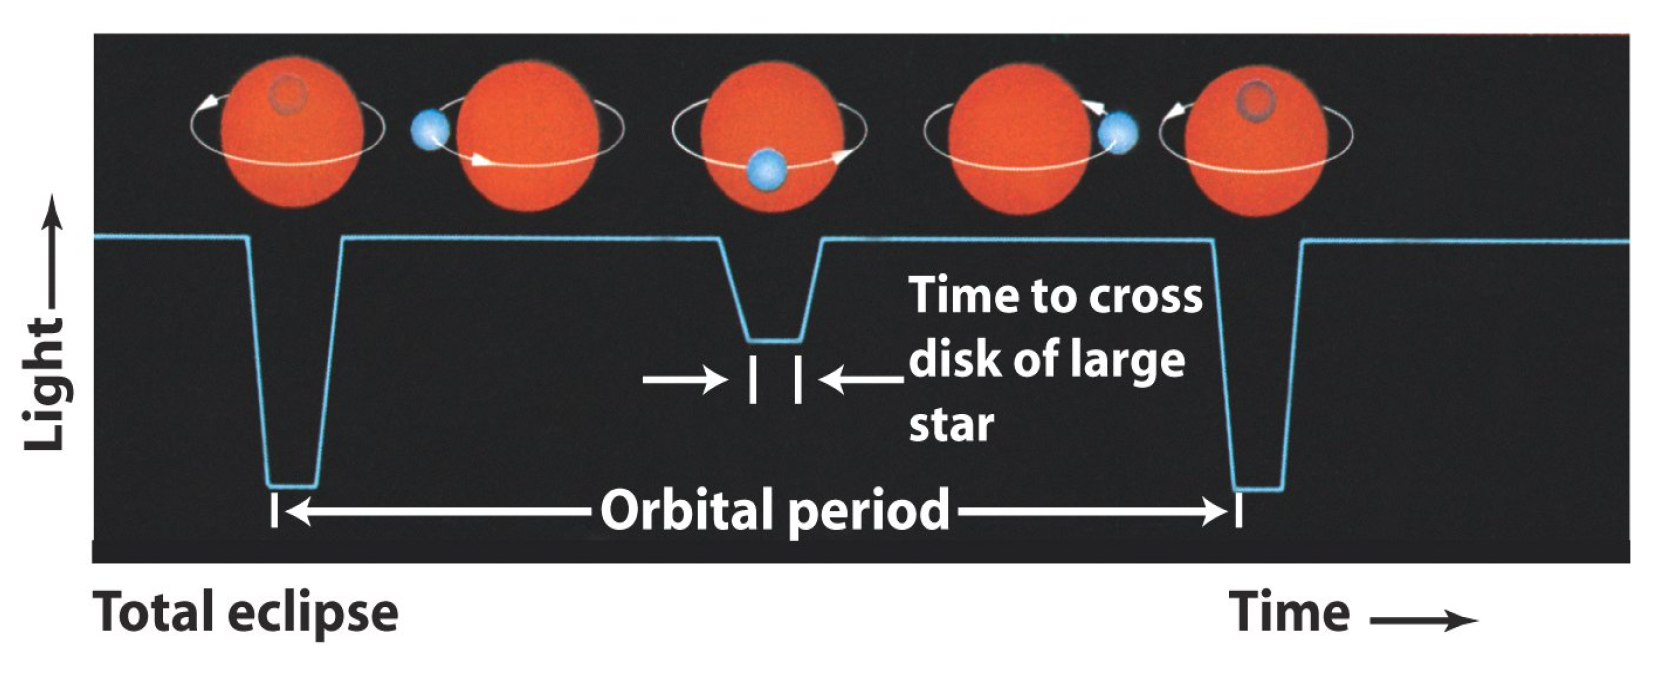
\includegraphics[width=\linewidth]{Figures/eclipsing_binary.png}
            \caption{Καμπύλη φωτός για ένα εκλειπτικά διπλό σύστημα αστέρων. Όταν ο αμυδρότερος αστέρας καλύπτει τον λαμπρότερο έχουμε το \textit{πρωτεύον ελάχιστο}. Στην αντίθετη περίπτωση έχουμε το \textit{δευτερεύων ελάχιστο}.}
            \label{fig:eclipsing_binary}
        \end{figure}
        
    Και σε αυτή την περίπτωση δεν μπορούμε να υπολογίσουμε τη μάζα κανενός από τους αστέρες του συστήματος. Από την καμπύλη φωτός όμως (σχήμα \ref{fig:eclipsing_binary}) μπορούμε να υπολογίσουμε την κλίση της τροχιάς, τις ακτίνες των μελών του ζεύγους και τον λόγο των φωτεινοτήτων των δύο αστέρων. Αν επιπροσθέτως τα δύο αστέρια ανήκουν στην κύρια ακολουθία μπορούμε να υπολογίσουμε και τον λόγο των μαζών από τη σχέση μάζας-φωτεινότητας.
    
    \item \textbf{Αστρομετρικά διπλοί αστέρες (astrometric binaries)}\\
    Στη κατηγορία αυτή κατατάσσονται τα μη-οπτικώς διπλά συστήματα αστεριών, των οποίων ο αμυδρός συνοδός αστέρας εντοπίζεται μόνο μέσω των δυναμικών επιδράσεων του πάνω στην τροχιά του πρωτεύοντος αστέρα. Ουσιαστικά παρατηρούμε μόνο ένα άστρο, επειδή όμως η κίνηση στην τροχιά του παρουσιάζει παλινδρομήσεις, συμπεραίνουμε ότι υπάρχει αμυδρός συνοδός.
    
    \item \textbf{Φασματικά διπλοί αστέρες (spectral binaries)}\\
    Αν οι τυπικές ταχύτητες περιφοράς των μελών ενός διπλού συστήματος ή/και η γωνία κλίσης $i$ είναι πολύ μικρή, τότε δεν είναι δυνατόν να ανιχνευθεί η μετατόπιση Doppler των φασματικών γραμμών και επομένως το σύστημα δεν αναγνωρίζεται ως φασματοσκοπικά διπλός αστέρας. Παρόλα αυτά, αν τα δύο μέλη έχουν σημαντικά διαφορετικά φάσματα (ανήκουν δηλαδή σε διαφορετικούς φασματικούς τύπους) και συγκρίσιμες λαμπρότητες (έτσι ώστε και τα δύο φάσματα να είναι ορατά), τότε το σύστημα μπορεί να αναγνωριστεί ως φασματικά διπλός αστέρας.
    
    Είναι φανερό ότι οι φασματικά διπλοί αστέρες διαφέρουν από τους φασματοσκοπικά διπλούς στο ότι στους πρώτους δεν παρατηρείται μετατόπιση Doppler των γραμμών. Κανένα στοιχείο δεν μπορεί να βρεθεί για τους φασματικά διπλούς αστέρες αφού δεν παρατηρούμε σ' αυτούς κανένα φαινόμενο που να εμφανίζει χρονική μεταβολή.
\end{enumerate}

\subsection{Βασικοί υπολογισμοί}

\subsubsection{Υπολογισμός στοιχείων τροχιάς}
Μετατρέποντας τη \textit{σχετική φαινόμενη τροχιά} σε \textit{σχετική πραγματική τροχιά}, υπολογίζουμε:
\begin{eqnarray*}
    \epsilon_{\pi} &=& \ \text{εκκεντρότητα} \\
    \alpha_{\pi} &=& \ \text{μεγάλος γωνιώδης ημιάξονας σε AU} \\
    i &=& \ \text{γωνία κλίσης}
\end{eqnarray*}

Αν γνωρίζουμε την παράλλαξη $\pi$, τότε υπολογίζουμε τον μεγάλο ημιάξονα $\alpha$ σε AU
\begin{equation}
    \alpha = \frac{\alpha_{\pi}}{\pi}
\end{equation}

\subsubsection{Υπολογισμός αθροίσματος μαζών}
Από τον 3ο νόμο του Kepler (σχέση \eqref{eq:Kepler_third_law}) έχουμε ότι 
$$M_1 + M_2 \simeq \frac{\alpha ^3}{P^2}$$ όπου $\alpha$ είναι ο μεγάλος ημιάξονας σε AU και $P$ η περίοδος του συστήματος.


\subsubsection{Υπολογισμός μαζών $M_1. M_2$}
Για φωτεινά διπλά συστήματα με σχετικά μεγάλη γωνιώδη απόσταση $\alpha_{\pi}$, μπορούμε να υπολογίσουμε και την \textit{απόλυτη φαινόμενη τροχιά} για καθένα από τα δύο μέλη. Άρα υπολογίζουμε δύο ημιάξονες $\alpha_1, \alpha_2$.

Από τον ορισμό του ΚΜ του συστήματος (σχέση \eqref{eq:center_mass}) και σε συνδυασμό με τον υπολογισμό του αθροίσματος $M_1 + M_2$ προκύπτουν οι μάζες $M_1, M_2$ για κάθε αστέρα.

\subsubsection{Δυναμικές παραλλάξεις}
 Από τις σχέσεις:
 \begin{eqnarray*}
    M_1 + M_2 &=& \frac{\alpha^3}{P^2} \\\\
    \alpha &=& \frac{\alpha_{\pi}}{\pi} 
 \end{eqnarray*}
 προκύπτει ότι:
 \begin{equation}
     \alpha_{\pi} = \pi \left[ (M_1 + M_2)P^2 \right]^{1/3}
 \end{equation}
 
 Αν οι δύο αστέρες ανήκουν στην κύρια ακολουθία, τότε για τον καθένα ισχύει ο νόμος μάζας-φωτεινότητας $L = f(M)$. Οπότε λύνουμε επαναληπτικά το σύστημα:
 
 \begin{eqnarray*}
    \pi &=& \alpha_{\pi} \left[ (M_1 + M_2)P^2 \right]^{-1/3} \\\\
    L_1 &=& f(M_1) \\\\
    L_2 &=& = f(M_2)
 \end{eqnarray*}
 για $\pi, M_1, M_2$ ξεκινώντας από κάποια εκτίμηση για το $M_1 + M_2$.  




\subsection{Στενά διπλά συστήματα \& απώλεια μάζας}
Κατά τη διάρκεια της ζωής τους, τα αστέρια χάνουν μάζα η οποία εμπλουτίζει τον μεσοαστρικό χώρο μέσω δύο διακασιών:
\begin{enumerate}[label=(\alph*)]
    \item \textbf{Συνεχώς}, μέσω των αστρικών ανέμων. Η μάζα που μπορεί να χαθεί με αυτόν τον τρόπο εξαρτάται από τη μάζα του αστέρα καθώς και το στάδιο της εξέλιξής του ($\dot{M}_{\text{Giant}} > \dot{M}_{MS}$).
    \item \textbf{Εκρηκτικώς}, μέσω καινοφανών και υπερκαινοφανών εκρήξεων.
\end{enumerate}

{\color{red} \hrule}
Στην περίπτωση ενός στενού διπλού συστήματος, οι αλληλεπιδράσεις μεταξύ των μελών μπορεί να οδηγήσει σε μεταφορά μάζας από το ένα αστέρι στο άλλο, επηρεάζοντας με αυτόν τον τρόπο την δομή, την μάζα, την γωνιακή στροφορμή καθώς και την τελική κατάσταση των αστέρων του συστήματος.
{\color{red} \hrule}

Όταν έχουμε ένα διπλό σύστημα, το πρόβλημα των πολλών σωμάτων (n-body problem) εκφυλίζεται στο ``περιορισμένο κυκλικό πρόβλημα των τριών σωμάτων'' (circular restricted three-body problem), με το ενεργό (effective) δυναμικό να δίνεται από τη σχέση:
\begin{equation}
    \label{eq:effective_potential}
    \Phi = - G \left( \frac{M_1}{r_1} + \frac{M_2}{r_2} \right) - \frac{1}{2} \Omega^2 r_3^2
\end{equation}
όπου  $r_1, r_2$ είναι οι αποστάσεις από το κέντρο των αστέρων $M_1, M_2$ αντίστοιχα, $\Omega$ είναι η τροχιακή γωνιακή ταχύτητα και $r_3$ είναι η απόσταση του άξονα περιστροφής τους συστήματος.

Η ποσότητα $\displaystyle V_g = - G \left( \frac{M_1}{r_1} + \frac{M_2}{r_2} \right)$ είναι ουσιαστικά το βαρυτικό δυναμικό ενώ το $\displaystyle V_F = - \frac{1}{2} \Omega^2 r_3^2$ περιγράφει το ``δυναμικό'' της φυγόκεντρου δύναμης. 

Αν απαιτήσουμε η συνολική δύναμη που ασκείται σε ένα δοκιμαστικό σωματίδιο, $m$, να είναι μηδέν: $$\boldsymbol{F_t} = - \nabla \Phi = 0$$
τότε η εξίσωση \eqref{eq:effective_potential} δίνει πέντε λύσεις όπου η βαρυτική δύναμη εξισορροπεί την φυγόκεντρο δύναμη που προκαλείται από τη σχετική κίνηση των δύο αστέρων του ενός γύρω από τον άλλον. Τα σημεία για τα οποία ισχύει αυτό, δηλαδή τα σημεία τα οποία έχουν μηδενική στιγμιαία ταχύτητα ονομάζονται \textit{σημεία Lagrange}, ($L_n, n = 1, \dots, 5$). Άρα αν το δοκιμαστικό σωματίδιο τοποθετούνταν σε κάποιο από αυτά τα σημεία, θα διατηρούσε τη θέση του σε σχέση ως προς τα δύο αστέρια.

Το σύνολο των σημείων μηδενικής ταχύτητας συγκροτεί μία ομάδα κλειστών επιφανειών, τις οποίες ονομάζουμε \textit{επιφάνειες μηδενικής ταχύτητας} (zero velocity surfaces) και περνούν από τα σημεία Lagrange. Η τομή μιας τέτοιας επιφάνειας μηδενικής ταχύτητας (ή ισοδυναμική επιφάνεια καθώς περιλαμβάνει όλα τα σημεία του συστήματος που μοιράζονται την ίδια τιμή του δυναμικού $\Phi$) με κάποιο συγκεκριμένο επίπεδο ονομάζεται \textit{καμπύλη μηδενικής ταχύτητας} (zero velocity curve). Συνήθως σαν επίπεδο τομής επιλέγεται το επίπεδο της σχετικής τροχιάς των δύο αστέρων του συστήματος (σχήμα \ref{fig:eq_sur}).
\\
{\color{red} \hrule}
Οι επιφάνειες μηδενικής ταχύτητας είναι σημαντικές γιατί ορίζουν τα όρια (boundaries) των περιοχών από τις οποίες το δοκιμαστικό σωματίδιο είναι δυναμικά αποκλεισμένο. Με άλλα λόγια, κάθε αστέρας ελέγχει βαρυτικά μόνο έναν περιορισμένο χώρο που καθορίζεται από μία ισοδυναμική επιφάνεια.
{\color{red} \hrule}

\begin{figure}[h]
   \centering
\begin{subfigure}[h]{0.45\textwidth}
	\centering
   	 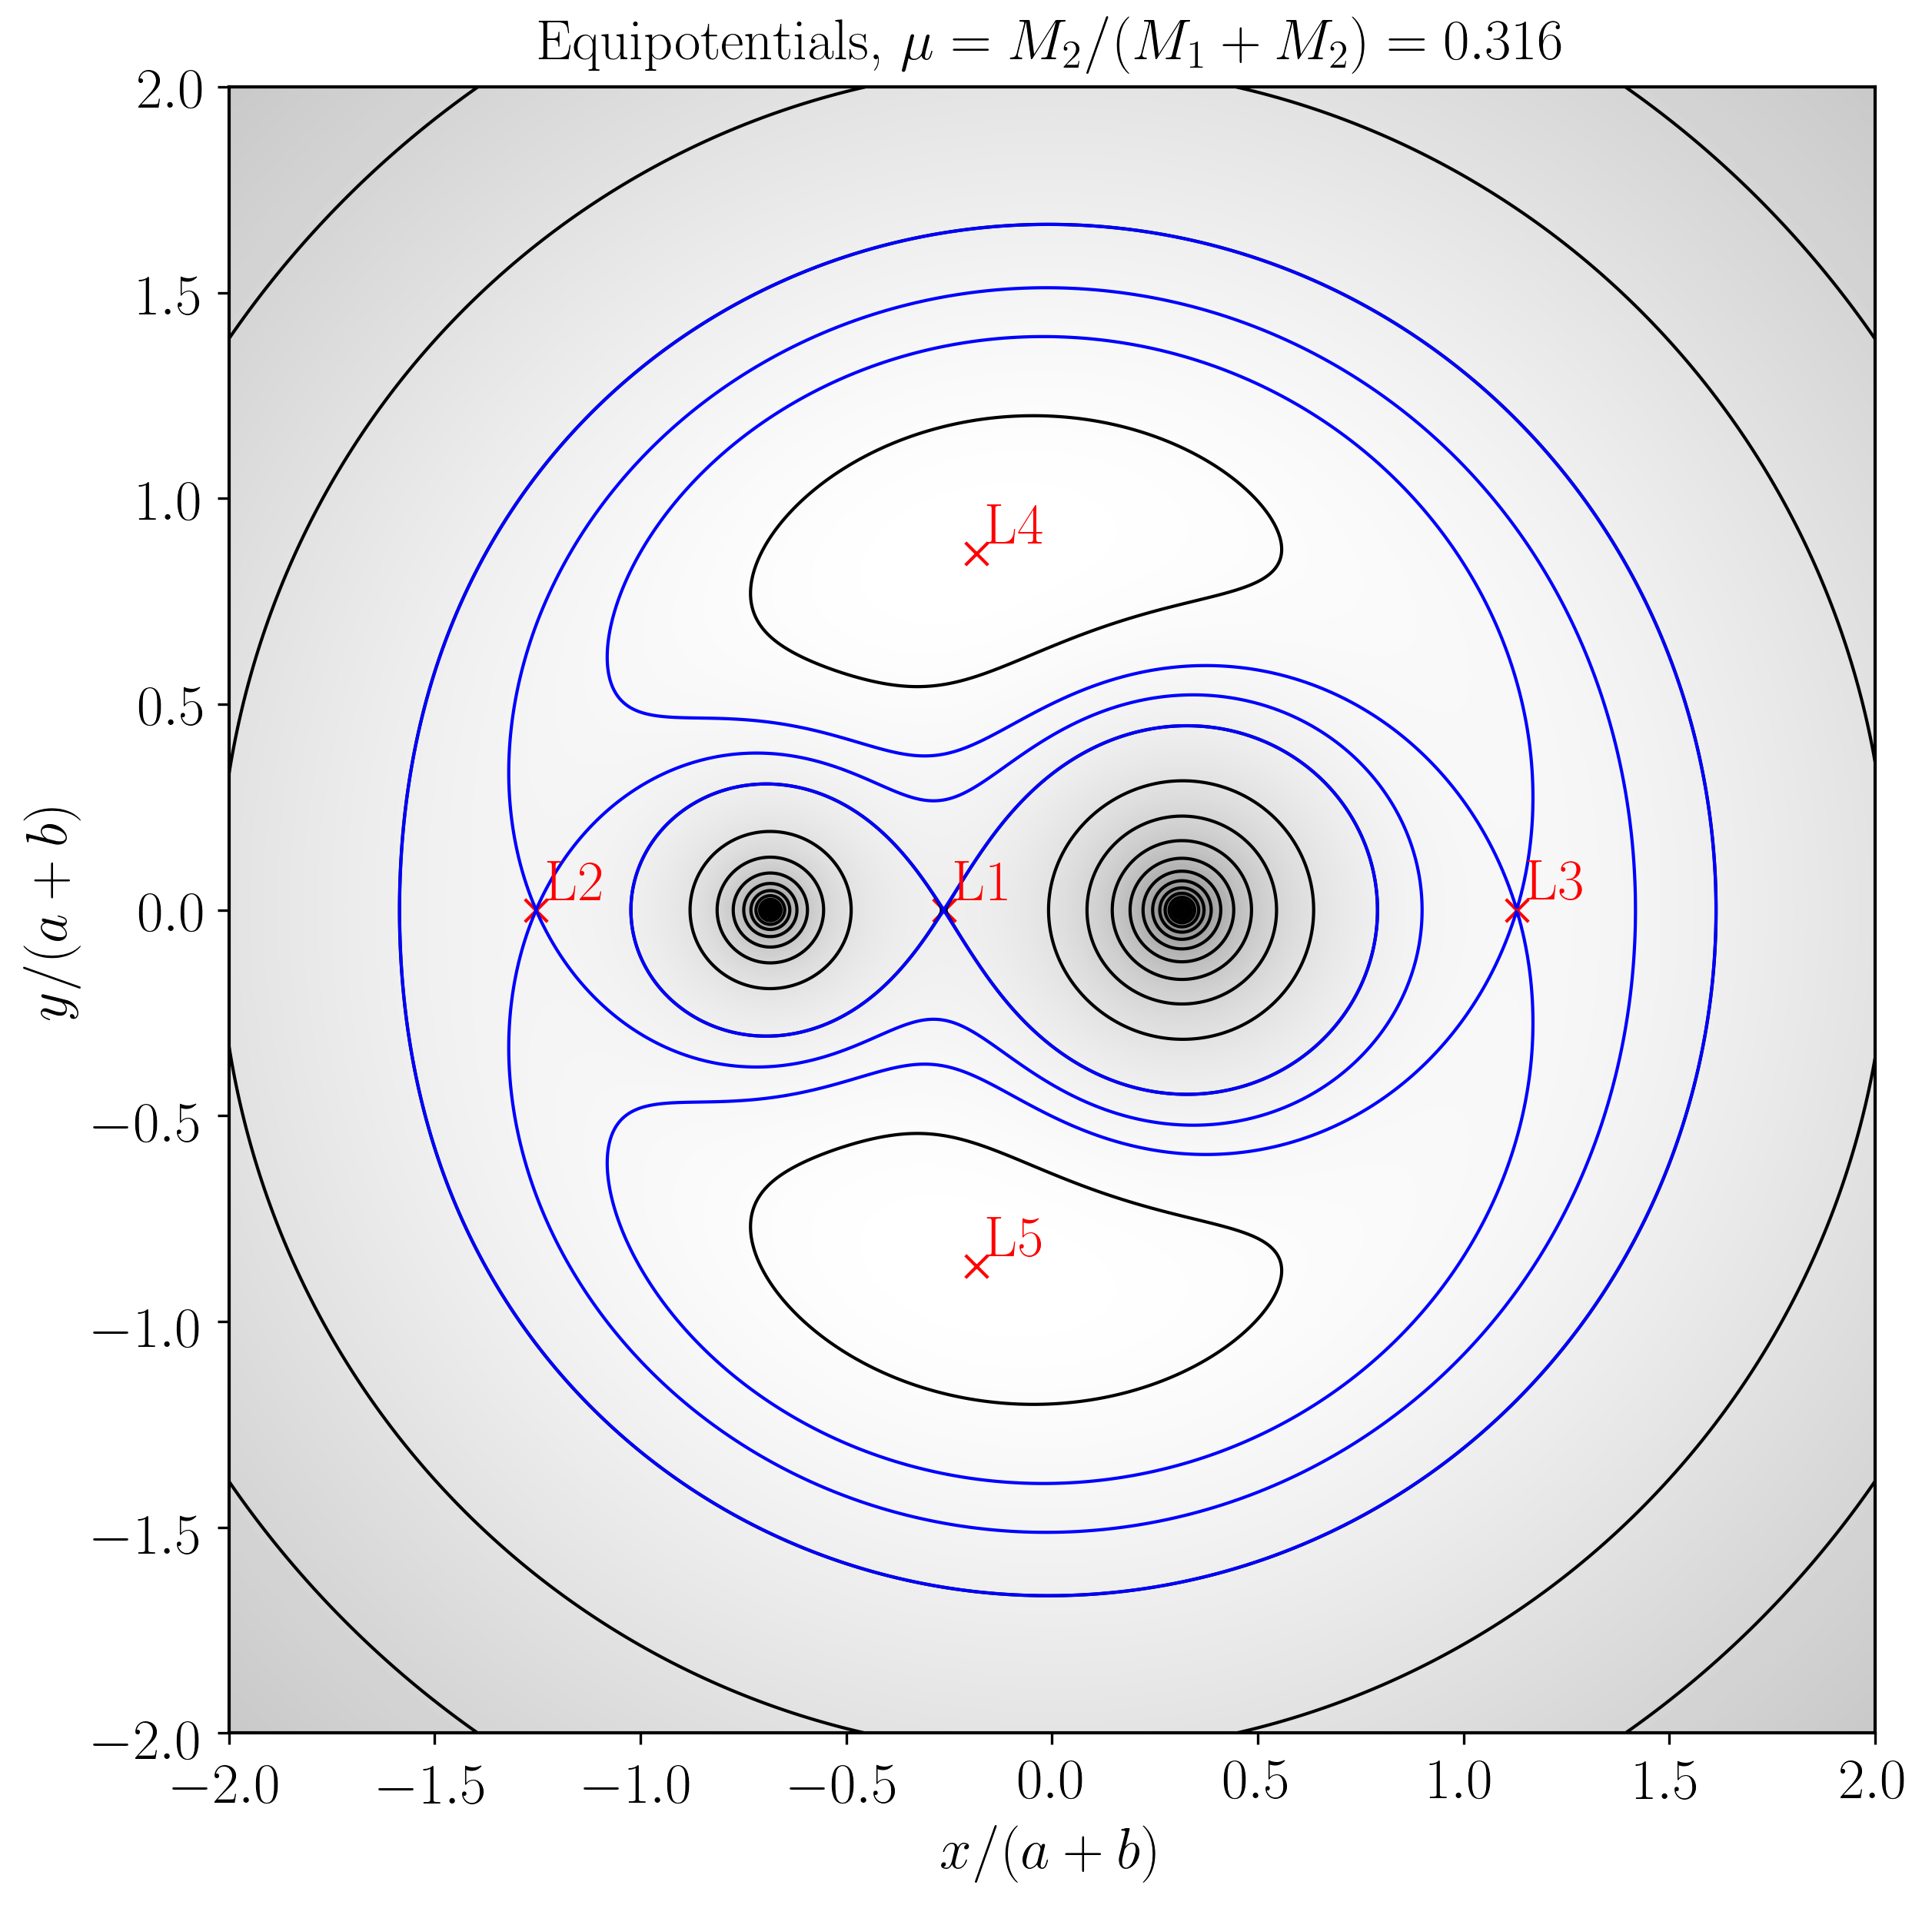
\includegraphics[width = \linewidth]{Figures/equipotentials_mu_0_316.png} 
\end{subfigure}
\begin{subfigure}[h]{0.535\textwidth}
	\centering
	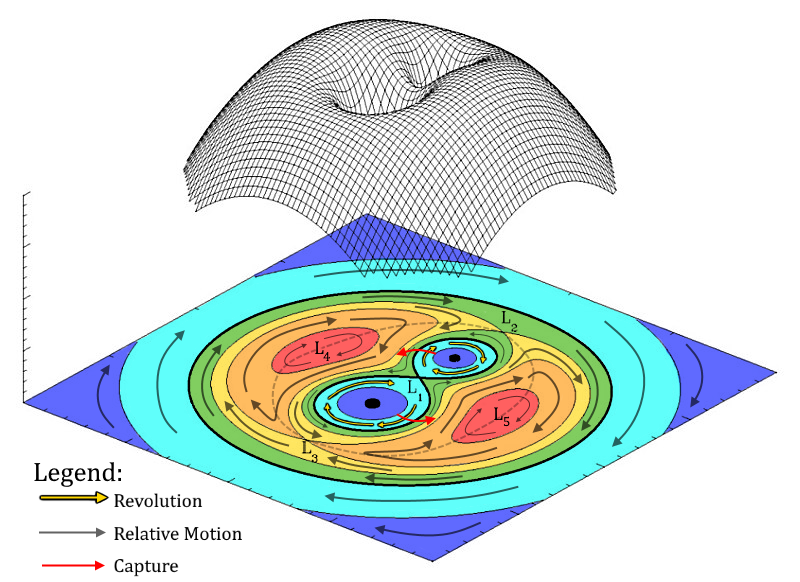
\includegraphics[width = \linewidth]{Figures/RochePotential_-_Colorized.png} 
    \end{subfigure}
    \caption{\textbf{Left panel}: Equipotential lines in the orbital plane of a rotating binary system, with a reduced mass ratio of $\mu = 0.316$. In this setup, $M_1$ is the more massive and is located at $x = +a$, whilst $M_2$ is the less massive and is at $x = -b$. The inner equipotential surface that passes from the $L_1$ Lagrangian point, defines the ``teardrop''-shaped Roche-lobes, one for each star. Contour lines passing through the Lagrange points are marked with blue colour. \textbf{Right Panel}: 3D representation of equipotential surfaces.}
    \label{fig:eq_sur}
\end{figure}

Στο σχήμα \ref{fig:eq_sur} κάθε καμπύλη μηδενικής ταχύτητας έχει παρουσιαστεί με διαφορετικό χρώμα. Από τα πέντε σημεία Lagrange, το $L_1$ παίζει σημαντικό ρόλο στην εξέλιξη των διπλών συστημάτων καθώς η ισοδυναμική επιφάνεια που περνάει από αυτό ορίζει τους (ανεξάρτητους μεταξύ τους) \textit{λοβούς Roche} και κάθε ένας από αυτούς περιβάλλει έναν αστέρα του συστήματος.

Η επιφάνεια μηδενικής ταχύτητας που περνάει από το $L_1$ έχει ένα ιδιαίτερο χαρακτηριστικό: όλες οι επιφάνειες μηδενικής ταχύτητας που περιβάλλουν ένα μόνο σώμα, βρίσκονται μέσα στον αντίστοιχο λοβό Roche, ενώ όλες οι επιφάνειες μηδενικής ταχύτητας που βρίσκονται έξω από τους λοβούς Roche περιβάλλουν και τα δύο σώματα. Έτσι, ένα δοκιμαστικό σωματίδιο που βρίσκεται μέσα στο λοβό Roche ενός μέλους του διπλού συστήματος ``ανήκει'' βαρυτικά σε αυτόν τον αστέρα. Αντίθετα, ένα σωματίδιο που βρίσκεται έξω και από τους δύο λοβούς Roche ``ανήκει'' βαρυτικά και στους δύο αστέρες, αφού κινείται σε τροχιά που είναι δυνατόν να περιβάλλει και τους δύο. Οι τροχιές αυτές δεν είναι κωνικές τομές (κύκλοι, ελλείψεις, παραβολές, υπερβολές ή ευθείες).

Με βάση το λόγο της ακτίνας του κάθε αστέρα ως προς την ακτίνα του δικού του λοβού ($R_L$), τα διπλά συστήματα χωρίζονται στις εξής κατηγορίες:

\subsubsection{Αποχωρισμένα (detached binaries)}
Είναι ένα διπλό σύστημα στο οποίο ο κάθε ένας αστέρας βρίσκεται εξ' ολοκλήρου μέσα στον δικό του λοβό Roche και εξελίσσονται σχεδόν ανεξάρτητα ο ένας από τον άλλον. Ισχύει δηλαδή ότι $r_1 < R_{L,1}$ και $r_2 < R_{L,2}$ όπου $r_1, r_2$ οι ακτίνες των δύο αστέρων.

\subsubsection{Ημιαποχωρισμένα (semidetached binaries)}
Αυτά είναι τα συστήματα στα οποία μόνο ο ένας από τους δύο αστέρες ``γεμίζει'' τον λοβό Roche του (δηλαδή $r_1 < R_{L,1}$ και $r_2 \approx R_{L,2}$). Αυτό μπορεί να συμβεί σε μετεγενέστερα εξελικτικά στάδια στη διάρκεια ζωής ενός αστέρα, όταν μπει στη φάση των γιγάντων,
Έκεί, η ακτίνα του μεγαλώνει σε τόσο βαθμό όπου ο όγκος του αστέρα είναι συγκρίσιμος με  τον όγκο που ορίζει ο λοβός Roche του.

Σε αυτή την περίπτωση έχουμε εκροή μάζας από αυτόν τον αστέρα προς τον συνοδό του διαμέσου το εσωτερικού $L_1$ σημείο Lagrange. Η προσαύξηση του υλικού γίνεται με τον σχηματισμό ενός \textit{δίσκου επισυσσώρευσησ/προσαύξησης} και όχι με το να πέφτει απευθείας πάνω στον συνοδό αστέρα. Αυτό συμβαίνει διότο το υλικό που εκρύεται έχει την ίδια στροφορμή με τον αστέρα-δότη και εκτός αν υπάρχουν μη-συντηρητικές μηχανισμοί για να αφαιρέσουν ένα ποσό από τη στροφορμή του αερίου που εκρύεται, αυτό θα συνεχιστεί να περιφέρεται γύρω από τον συνοδό αστέρα. Για να καταφέρει να πέσει πάνω στον αστέρα, η ύλη πρέπει να χάσει στροφορμή από την εσωτερική τριβή (ιξώδες). Αυτή η εσωτερική τριβή του αερίου το αναγκάζει να θερμανθεί και να ακτινοβολεί (X-ray binary).

Η υπερχείλιση του αστέρα μέσα από τον λοβό του Roche οδηγεί σε σημαντική μείωση της μάζας του αστέρα και επηρεάζει τη μετέπειτα εξέλιξή του. Πέρα από αυτόν τον μηχανισμό όμως, μπορούμε να έχουμε μεταφορά μάζας με προσαύξηση από τον \textit{αστρικό άνεμο} του θερμότερου αστέρα προς τον ψυχρότερο. Παρόλα αυτά, η μεταφορά μάζας με αυτόν τον τρόπο δεν είναι το ίδιο αποδοτική όσο η υπερχείλιση του λοβού Roche.

\subsubsection{Εν επαφή (contact binary)}
Ένα διπλό σύστημα λέμε ότι είναι σε επαφή ότα και τα δύο αστέρια ``γεμίζουν'' τους λοβούς τους (δηλαδή $r_1 \approx R_{L,1}$ και $r_2 \approx R_{L,2}$). Σε αυτή την περίπτωση, το σύστημα μοιράζεται μία κοινή ατμόσφαιρα (common envelope, σχήμα \ref{fig:binary_cases}) η οποία μπορεί να εκδιωχθεί στερώντας έτσι από το σύστημα ένα σημαντικό μέρος της μάζας του.

\begin{figure}
    \centering
    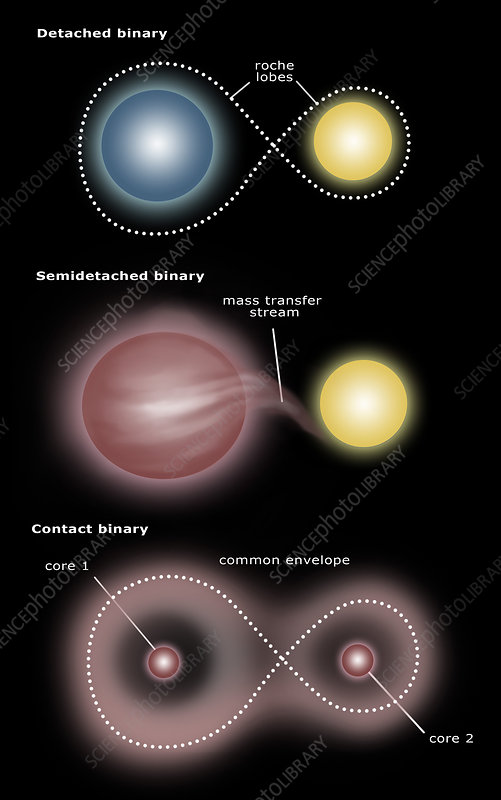
\includegraphics[scale=0.3]{Figures/binary_cases.jpeg}
    \caption{Κατηγορίες διπλών συστημάτων βάσει του ποσοστού πλήρωσης των λοβών Roche.}
    \label{fig:binary_cases}
\end{figure}

Σε αυτό το σημείονα διευκρινήσουμε ότι δεν υπάρχει αναλυτική έκφραση για το μέγεθος του λοβού Roche σε ένα διπλό σύστημα. Παρόλα αυτά έχει προταθεί μια αριθμητική προσέγγιση της ακτίνας του λοβού Roche μέσω της σχέσης:
$$\frac{R_L}{a} = \frac{0.49q^{2/3}}{0.6q^{2/3} + \ln (1 + q^{1/3})}$$
όπου $a$ είναι ο τροχιακός διαχωρισμός (orbital separation) του συστήματος και $\displaystyle q \equiv \frac{M_{\text{donor}}}{M_{\text{accretor}}}$ είναι ο λόγος των μαζών των μελών του συστήματος.
Αυτές είναι και οι δύο πιο σημαντικές παράμετροι για να ακολουθήσουμε την εξέλιξη του συστήματος.













\section{Μεταβλητοί αστέρες}
\subsection{Περιοδικοί}
\subsubsection{Κηφείδες}
\subsubsection{RR Lyrae}
\subsubsection{Μακροπερίοδοι}

\subsection{Μη-περιοδικοί}
\subsubsection{Ανώμαλοι - T Tauri}
\subsubsection{Ανώμαλοι - Αστέρες εκλάμψεων}
\subsubsection{Ανώμαλοι - R Coronae Borealis}
\subsubsection{Καταστροφικοί - Καινοφανείς}
\subsubsection{Καταστροφικοί - Υπερκαινοφανείς I}
\subsubsection{Καταστροφικοί - Υπερκαινοφανείς II}
